\documentclass[aps,prx,reprint,amsmath,amssymb,floatfix,nofootinbib,superscriptaddress]{revtex4-2}

\usepackage{graphicx}
\usepackage{dcolumn}
\usepackage{bm}
\usepackage{hyperref}
\usepackage{booktabs}
\usepackage{array}
\usepackage{xcolor}

\hypersetup{
  colorlinks=true,
  linkcolor=blue!50!black,
  citecolor=blue!50!black,
  urlcolor=blue!50!black,
  pdftitle={A dichotomous Leggett-Garg witness for braid-representation density in SU(2)k: exact at d=2, dimension-limited at d>=3},
  pdfauthor={Berkay Yuksel Sayim},
  pdfsubject={quant-ph; SU(2)_k anyons; Leggett-Garg inequality; braid-representation density},
  pdfkeywords={Leggett-Garg inequality, Luders bound, SU(2)k anyons, Fibonacci anyons, braid group density,
               Jones representations, topological quantum computation, temporal quantum correlations,
               dimension witness, modular tensor category, universality}
}

\begin{document}
\setcounter{secnumdepth}{3} % v1.1 series convention (1a/1b/2/3 consistency)

\title{A dichotomous Leggett--Garg witness for braid-representation density in
$\mathrm{SU}(2)_k$: exact at $d=2$, dimension-limited at $d \ge 3$}

\author{Berkay Y\"uksel Sayim}
\email{berksa@tutamail.com}
\affiliation{Independent Research, Germany\\
\href{https://orcid.org/0009-0004-4993-7352}{ORCID: 0009-0004-4993-7352}}

\date{2026-07-22}

\begin{abstract}
Whether a \emph{temporal} (Leggett--Garg) measurement can certify the computational
power of an anyonic braid representation---its \emph{density} in the unitary group,
the property underlying universal topological quantum computation---has, to our
knowledge, not been studied. We give a complete operational characterization of when the dichotomous
L\"uders--Leggett--Garg witness $K_3 = 2\,C(B) - C(B^2)$ resolves braid-representation
density across the $\mathrm{SU}(2)_k$ family. At $d=2$ (the spin-$\tfrac12$ fusion
space) the witness resolves density \emph{exactly}: it saturates the
dimension-independent L\"uders bound $3/2$ on every dense representation and stays
strictly below it on the finite ones, which on this minimal-rank, one-qubit space
occur precisely at $k \in \{2,4,8\}$---a sharp threshold distinct from the all-rank
finite set $k \in \{1,2,4\}$ of Freedman--Larsen--Wang and Kuperberg. The $k=4$
representation is structurally inert ($K_3 = 1$ for
\emph{every} measurement axis) despite a \emph{larger} quantum dimension than $k=3$,
its braid image being finite; and $k=8$ is pinned at $3/\sqrt5$ (at $Q=\hat z$; $1.427$
axis-optimized). Both follow from the
underlying $\mathrm{SO}(3)$ geometry. At $d \ge 3$ the \emph{same} witness ceases to
resolve density---it saturates $3/2$ even on finite representations---and we trace
this to the extra dimension itself, not to any particular braid angle. We frame the
resulting no-go question---whether \emph{every} such witness is density-blind at
$d \ge 3$---as an open problem.
\end{abstract}

\maketitle

\section{Introduction}
\label{sec:intro}

Anyonic braiding is universal for quantum computation exactly when the braid-group
representation is \emph{dense} in the relevant (projective) unitary
group~\cite{Kup,FLW}. Density is therefore the structural property one would most like
to \emph{certify operationally}. Existing operational benchmarks for anyonic
computational power are \emph{spatial}: Howard and Vala use a CHSH--Bell violation as
a universality benchmark for Ising anyons~\cite{HV}. The complementary \emph{temporal}
route---a Leggett--Garg (LG) test~\cite{LeggettGarg1985,EmaryLambertNori2014}, which
probes the nonclassicality of a \emph{single} system measured sequentially---has, to
our knowledge, never been connected to braid-representation density. A companion
Letter reports the isolated Fibonacci ($k=3$, $d=2$) case of this LG-density
connection~\cite{Sayim2026LGI}; the present work is supplemented by that Letter
and generalizes the connection to density across the complete
$\mathrm{SU}(2)_k$ family.

Here we characterize that connection completely, across the \emph{entire}
$\mathrm{SU}(2)_k$ anyon family resolved by level $k$ and anyon spin $j$. We find a
clean two-sided result. At $d=2$ the witness is a faithful density probe with sharp,
fully characterized structure; at $d \ge 3$ it stops resolving density, for a reason
we pin down. The negative half is not an aside: it converts ``we found a witness that
works at $d=2$'' into ``we know exactly where this witness works, where it stops, and
why,'' and pre-empts the obvious generalization question instead of leaving it open.

We are careful about what is and is not claimed (Sec.~\ref{sec:prior}): the $3/2$
L\"uders bound is established prior art~\cite{BMKG,BE} which we \emph{cite}, not claim;
the operational characterization of where \emph{this} witness tracks density is, to
the best of a full-text prior-art search, new.

\section{Setup}
\label{sec:setup}

\paragraph{The witness.}
For a three-time LG protocol with a dichotomic observable $Q$ ($Q^2 = I$,
eigenvalues $\pm 1$) measured under a single braid unitary $B$, with the \emph{L\"uders}
(degeneracy-preserving) update rule, the stationary three-time correlator combination is
\begin{equation}
  K_3 = 2\,C(B) - C(B^2),
  \qquad
  C(U) = \tfrac1d\,\mathrm{Re}\,\mathrm{Tr}\!\left[Q\,U\,Q\,U^{\dagger}\right],
\label{eq:K3}
\end{equation}
where $d$ is the dimension of the braid representation (the fusion space) and the
prefactor $1/d$ is the maximally mixed state $\rho = I/d$. The symmetrized
two-time correlator form $C = \tfrac12 \langle \{Q_i, Q_j\} \rangle$ for sequential
L\"uders measurements of a dichotomic observable is that of the temporal CHSH
scenario~\cite{Fri}; our $C(U)$ is its $\rho = I/d$ specialization. For a
general state $\rho$ we use the full sequential-L\"uders statistics, which yields a
witness operator $M$ with $K_3(\rho) = \mathrm{Tr}[\rho M]$; the state-optimized value
is $\rho\text{-opt} = \lambda_{\max}\!\big(\tfrac12 (M + M^{\dagger})\big)$ and the
maximally-mixed value is $\mathrm{Tr}[M]/d$.

\paragraph{The bound.}
Under L\"uders, $K_3 \le 3/2$ \emph{independently of dimension}~\cite{BMKG,BE}; the
bound can be exceeded (up to the algebraic value $3$) \emph{only} under the
degeneracy-breaking von-Neumann rule, which we do \emph{not} use~\cite{BE} (cf.\ the
arbitrary-spin construction of Ref.~\cite{MM}, Sec.~\ref{sec:prior}). We write
\emph{``fires'' $:=$ saturates $3/2$}. This precise meaning matters: $k=8$ at $d=2$
gives $K_3 > 1$ yet does \emph{not} saturate (Sec.~\ref{sec:d2}).

\paragraph{The family.}
$\mathrm{SU}(2)_k$ representations are indexed by level $k$ and spin $j$; the fusion
space of three anyons (chosen total charge) has dimension $d$, with
$j = \tfrac12 \to d = 2$ ($k \ge 2$), $j = 1 \to d = 3$ ($k \ge 4$),
$j = \tfrac32 \to d = 4$, $j = 2 \to d = 5$. ``Resolving density'' means: does the
witness value distinguish \emph{dense} representations (universal) from \emph{finite}
(nonuniversal) ones?

\paragraph{The engine.}
We use a projective $F/R$-symbol representation of $B_3$ (q-deformed $6j$/Racah),
which is phase-blind and therefore sees exactly the \emph{projective} braid image
(determinant phase removed)---the density notion relevant to a correlator-based
witness. This phase-blindness is appropriate, not a limitation: global phases are
physically irrelevant, and a correlator-based witness sees only the projective image
in any case. A gate-$0$ check reproduces the published $d=2$ values exactly, and the
Yang--Baxter relation holds to residual $\lesssim 10^{-15}$ across $d = 2,\ldots,5$
(Appendix~\ref{app:engine}).

\paragraph{The reported witness value.}
For a given representation, the witness value we report is the
supremum of $K_3(B)$ over the braid-group image $\rho(B_3)$,
maximized over the measurement axis; ``fires'' means this supremum
reaches $3/2$. It is this supremum over the image---not the value of
any single generator---that constitutes the density diagnostic: a
\emph{dense} image approaches $3/2$ as the supremum of a
never-exactly-attained set, whereas a \emph{finite} image attains
only a discrete set of values and can fall strictly short.

\section{Density resolution at $d=2$}
\label{sec:d2}

At $d=2$ (spin-$\tfrac12$) the witness resolves density, and the resolution is
\emph{biconditional in both directions} (Table~\ref{tab:d2}, Fig.~\ref{fig:k3d2}).

\begin{table}[b]
\caption{$K_3$ at $d=2$ (spin-$\tfrac12$) across $\mathrm{SU}(2)_k$. Dense levels
saturate the L\"uders bound $3/2$; the finite levels $k \in \{2,4,8\}$ (this
minimal-rank, one-qubit space; see Sec.~\ref{sec:d2}) stay strictly
below. Values are the axis/$Q$-optimized $K_3$; the $Q=\hat z$ column is shown where
it differs.}
\label{tab:d2}
\centering
\begin{tabular}{r c c c c c}
\toprule
$k$ & dense? & $|G|$ & $K_3(Q{=}\hat z)$ & $K_3$ (opt.) & sat.\ $3/2$? \\
\midrule
2  & no  & 48  & $1.000$ & $1.000$ & no  \\
3  & yes & --- & ---     & $1.4999$ & yes \\
4  & no  & 24  & $1.000$ & $1.000$ & no  \\
5  & yes & --- & ---     & $1.4997$ & yes \\
6  & yes & --- & ---     & $1.4999$ & yes \\
7  & yes & --- & ---     & $1.5000$ & yes \\
8  & no  & 120 & $3/\sqrt5 \approx 1.342$ & $1.427$ & no  \\
9  & yes & --- & ---     & $1.4999$ & yes \\
10 & yes & --- & ---     & $1.5000$ & yes \\
\bottomrule
\end{tabular}
\end{table}

\begin{figure}[t]
\centering
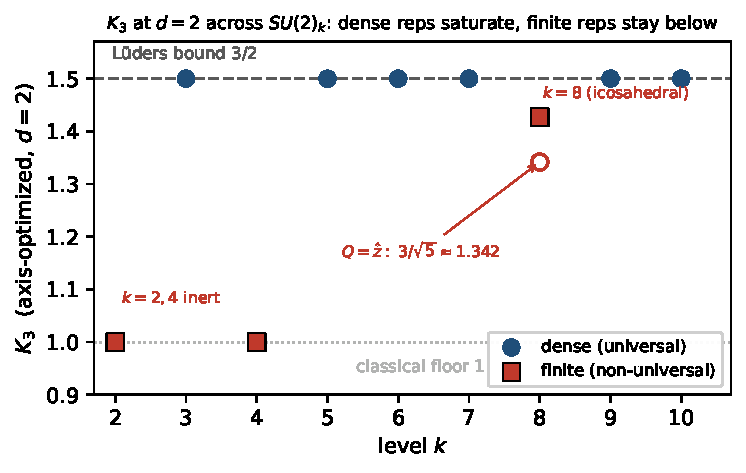
\includegraphics[width=\columnwidth]{paper4_fig1_K3_vs_k_d2.pdf}
\caption{$K_3$ at $d=2$ (spin-$\tfrac12$) across $\mathrm{SU}(2)_k$, axis-optimized
reading. Dense levels $k \in \{3,5,6,7,9,10\}$ saturate the L\"uders bound $3/2$; the
finite levels $k \in \{2,4,8\}$ (minimal-rank, one-qubit space) stay strictly below---$k=2,4$ at the classical floor
$1$, and $k=8$ at $1.427$ (its $Q=\hat z$ reading $3/\sqrt5 \approx 1.342$ is the open
marker). The closest finite representation, $k=8$, sits only $\approx 0.07$ below the
bound.}
\label{fig:k3d2}
\end{figure}

\noindent\emph{Forward} (dense $\to$ saturates): the dense levels
$k \in \{3,5,6,7,9,10\}$ all reach $3/2$ to the precision shown---the values approach
$3/2$ as the supremum of a dense (never exactly attained) image, with
finite-word/sampling estimates landing at $1.4997$--$1.4999$, while $k = 7, 10$ sit at
$3/2$ to machine precision ($|3/2 - K_3| \lesssim 10^{-14}$).
\emph{Backward} (saturates $\to$ dense, i.e.\ finite reps stay strictly below): the
finite levels are exactly $k \in \{2,4,8\}$, with $\mathrm{SU}(2)$ braid images the
binary octahedral group ($k=2$, order $48$), the binary tetrahedral group ($k=4$,
order $24$), and the binary icosahedral group ($k=8$, order $120$)---equivalently
$r = k+2 \in \{4,6,10\}$, the finite set at this minimal rank identified by
Freedman--Larsen--Wang~\cite{FLW}, with the underlying $B_3$
representation-theoretic machinery due to Tuba--Wenzl~\cite{TW} (classification of
$B_3$ representations) and Rowell--Tuba~\cite{RT} (finite-image criterion). We
emphasize that $\{2,4,8\}$
is the finite-image set specific to the $d=2$ (one-qubit, $B_3$) fusion space
considered here. This differs from the all-rank finite set $k \in \{1,2,4\}$
($r \in \{3,4,6\}$) of Freedman--Larsen--Wang and Kuperberg~\cite{FLW,Kup}: $k=1$
($r=3$) gives a one-dimensional representation, excluded from a qubit setting,
while $k=8$ ($r=10$) is the icosahedral borderline case---finite at minimal rank,
hence finite here at $d=2$, but dense at higher rank ($n \ge 5$), a resolution due
to Kuperberg~\cite{Kup}. On the $d=2$ space the finite set is therefore
$\{2,4,8\}$, not $\{1,2,4\}$; both statements are correct on their respective
domains. Since the engine is phase-blind it realizes the projective
($\mathrm{PSU}(2)\cong\mathrm{SO}(3)$) images, of orders $24$, $12$, $60$ for
$k=2,4,8$; the orders $|G|=48,24,120$ quoted above are the binary
($\mathrm{SU}(2)$) lifts. The identification is fixed geometrically: $\sigma_1$
acts as a $90^\circ$ ($4$-fold) rotation at $k=2$---forcing the octahedral group,
since the tetrahedral group has rotation angles $\{0^\circ,120^\circ,180^\circ\}$
only---as a $120^\circ$ rotation at $k=4$ (tetrahedral), and as a $144^\circ$
rotation at $k=8$ (icosahedral). These three angles are the finite-level instances
of the general sector-phase family $\delta^\ast(k) = \pi k/(k+2)$
($k=2\to90^\circ$, $k=4\to120^\circ$, $k=8\to144^\circ$); the $\sigma_1=144^\circ$
identification above is exactly $\delta^\ast(8)$. Their witness values stay below $3/2$: $k=2,4$ at $1.000$, and $k=8$ at
$3/\sqrt5 \approx 1.342$ ($Q=\hat z$) or $1.427$ (optimal)---both $< 3/2$. This
two-sided hold is the substance of the $d=2$ result, and (Sec.~\ref{sec:d3}) the
backward direction is exactly what no longer holds at $d \ge 3$.

As a corollary worth stating: at $d=2$ the witness operationally separates the
\emph{universal} Fibonacci model ($k=3$, dense---its $K_3$ approaching $3/2$ as the
supremum of a dense image) from the \emph{nonuniversal} finite levels
$k \in \{2,4,8\}$ (this minimal-rank space; Fibonacci anyons are $\mathrm{SU}(2)_3$); this separation is a
$d=2$ phenomenon, lost at $d \ge 3$.

\paragraph{Sharp finite set and the $k=4$ surprise.}
The finite set on this minimal-rank space is precisely $\{2,4,8\}$; in particular $k=4$ is not merely below
$3/2$ but \emph{structurally inert}: $K_3 = 1$ for \emph{every} measurement axis,
established by a closed argument $\max_U \lambda_{\max}(M(U)) = 1$ (an eigenvalue
argument, not sampling; $0$ of the $24$ group elements violate). This is
counterintuitive: $k=4$ sits at the floor \emph{despite a larger quantum dimension
than $k=3$} ($D_4 = \sqrt3 \approx 1.732 > D_3 = \varphi \approx 1.618$, with
$D_{1/2} = 2\cos[\pi/(k+2)]$)---its braid image being \emph{finite} (order $24$).
Large quantum dimension does not predict the witness response; density (here, its
absence) does.

\paragraph{The $k=8$ value (closed form).}
$K_3(k{=}8, \hat z) = 3/\sqrt5$ is proven in closed form from the icosahedral
structure: with $K_3 = f(\theta, p) = 1 + 2c - 2c^2 - 2pc(1-c)$ ($c = \cos\theta$,
$p = n_z^2$), the identity $f(c,1) = 1$ (the $2c-2c^2=2c(1-c)$ term cancels the
$-2pc(1-c)$ term exactly at $p=1$, for every $\theta$) kills all $\theta \notin
(0^\circ, 90^\circ)$,
leaving only the $A_5$ angle $72^\circ$; the minimizing axis overlap $n_z^2 = 1/5$ is
the icosahedral $5$-fold $\leftrightarrow 5$-fold angle ($\cos = 1/\sqrt5$). Here
$\hat z$ is taken along a $5$-fold axis of the icosahedral image---witnessed by
$\sigma_1$, which acts as a $144^\circ$ rotation about $\hat z$. A rotation about
the measurement axis has $n_z^2=1$, so by the identity $f(c,1)=1$ it contributes
$K_3=1$ regardless of angle; in particular $\sigma_1$ itself gives $K_3=1$ in this
frame, \emph{not} $3/\sqrt5$. The value $3/\sqrt5$ is instead realized by a
distinct group element---a $72^\circ$ rotation about a \emph{different} $5$-fold
axis, sitting at the icosahedral $5$-fold $\leftrightarrow 5$-fold separation
$\cos^{-1}(1/\sqrt5)$ from $\hat z$ ($n_z^2=1/5$). Among the $A_5$ rotation angles
$\{72^\circ,120^\circ,144^\circ,180^\circ\}$, only $72^\circ$ lies in
$(0^\circ,90^\circ)$, and $f(72^\circ,1/5) = +3/\sqrt5$ is the largest value
attained at fixed $Q=\hat z$ over the group; the $144^\circ$ element about the
same tilted axis gives the negative branch $f(144^\circ,1/5) = -3/\sqrt5$.

\emph{Correction to v1.0:} the first release associated the $K_3 = 3/\sqrt{5}$
maximum with the $144^\circ$ generator rotation about the measurement axis. As
derived above, rotations about the measurement axis yield $K_3 = 1$ for every
angle; the maximum instead arises from the $72^\circ$ rotation about a tilted
five-fold axis ($p = 1/5$). No numerical value is affected.

\paragraph{Mechanism (structural, not topological).}
$C(U)$ reduces to the $zz$-component of the $\mathrm{SO}(3)$ rotation $R(U)$, so $K_3$
is an $\mathrm{SO}(3)$-geometric quantity; $k=8 = 3/\sqrt5$ follows from icosahedral
geometry, and the $k=4$ floor from the absence of any tetrahedral-group rotation in
$(0^\circ, 90^\circ)$. This is representation theory / finite-subgroup geometry---not
topology.

\section{Loss of resolution at $d \ge 3$}
\label{sec:d3}

At $d \ge 3$ the same witness no longer separates dense from finite---under
\emph{either} state reading.

\paragraph{(a) Neutral ($\rho = I/d$) under-resolves.}
The maximally-mixed value has the closed form $(3d-1)/(2d)$ for odd $d$ and $3/2$ for
even $d$. For odd $d \ge 3$ this cap is \emph{below} $3/2$ ($d=3 \to 4/3$,
$d=5 \to 7/5$), and \emph{both dense and finite} representations reach it---e.g.\ at
$d=3$ the dense $k = 5,\ldots,10$ and the finite $(4,1)$ all sit at $4/3$. No
separation. This neutral no-resolution result is established for
\emph{odd} $d \ge 3$; for even $d \ge 4$ the neutral cap is again
$3/2$, as at $d=2$, and whether the neutral reading resolves density
there is left open. The targeted reading below over-resolves at all
$d \ge 3$, even and odd alike.

\paragraph{(b) Targeted ($\rho$-opt) over-resolves.}
The state-optimized value reaches $3/2$ for \emph{any} nontrivial dynamics at every
$d \ge 3$. Crucially it does so \emph{even for finite (nondense) representations}. We
verified this on three independent finite $d=3$ families (Table~\ref{tab:finite}).
Since dense $d=3$ reps also reach $1.500$ under $\rho$-opt, firing no longer
discriminates density. (All three live in the smallest nontrivial total-charge
sector; the apparent $d=3$-vs-$d=5$ multiplicity at $(8,2)$ is resolved in
Appendix~\ref{app:sectors}.)

\begin{table}[b]
\caption{The targeted witness fires ($K_3 = 3/2$) on \emph{finite} $d=3$
representations, verified on three independent families.}
\label{tab:finite}
\centering
\begin{tabular}{c c c c}
\toprule
finite rep $(k,j)$ & $|G|$ & targeted $K_3$ & fires? \\
\midrule
$(4,1)$  & $162$ & $1.500$ & yes \\
$(8,2)$  & $450$ & $1.500$ & yes \\
$(12,3)$ & $882$ & $1.500$ & yes \\
\bottomrule
\end{tabular}
\end{table}

All three directly-tested finite representations live at $d=3$; no finite $d=5$
representation was checked directly. No finite $d=5$ anyon representation exists to
test in the level range swept ($k \le 16$): the $(8,2)$ representation at $d=5$ is
itself dense. For $d \ge 5$ the result therefore rests on the closed-form neutral
cap $(3d-1)/(2d)$ (computed through $d=7$) together with the dimension mechanism
below---\emph{shown} on three finite $d=3$ reps and structurally expected, rather
than directly verified, at higher $d$.

\paragraph{State-dependence appears only at $d \ge 3$.}
At $d=2$ the neutral and targeted readings \emph{coincide} (state-independent:
$k=4 \to 1.0/1.0$, $k=8 \to 1.427/1.427$); they \emph{split only from $d \ge 3$ on}.
The witness change between the $d=2$ and $d \ge 3$ analyses is therefore not a hidden
assumption swap---at $d=2$ there is nothing to swap.

\paragraph{Mechanism: the extra dimension, not a braid angle.}
Take the \emph{same} one-parameter rotation $R_y(\theta)$ and compare it as a $d=2$
unitary versus the same rotation embedded in $d=3$ as $R_y(\theta) \oplus 1$. The
targeted witness is angle-dependent at $d=2$ but angle-independent at $d=3$
(Table~\ref{tab:nail})---two disjoint code paths (an algebraic $G_{\mathrm{eff}}$ form
and a direct sequential-L\"uders solver) agree exactly. The extra dimension supplies
the spectral freedom to reach $3/2$ regardless of the braid angle. This refutes the
tempting reading that the witness merely re-uses a $d=2$-optimal $\sim 60^\circ$
rotation inside a sub-block: at $d=3$, $72^\circ/90^\circ/100^\circ$ fire equally. It
is the dimension, not the angle.

\begin{table}[t]
\caption{Dimension nail: the same rotation $R_y(\theta)$ at $d=2$ versus
$R_y(\theta) \oplus 1$ at $d=3$. The targeted witness is angle-dependent at $d=2$ but
fires for every angle at $d=3$.}
\label{tab:nail}
\centering
\begin{tabular}{c c c}
\toprule
$\theta$ & $d=2$ & $d=3 \oplus \mathrm{triv}$ \\
\midrule
$60^\circ$  & $1.500$ (fires) & $1.500$ (fires) \\
$72^\circ$  & $1.427$         & $\mathbf{1.500}$ (fires) \\
$90^\circ$  & $1.000$         & $\mathbf{1.500}$ (fires) \\
$100^\circ$ & $1.000$         & $\mathbf{1.500}$ (fires) \\
\bottomrule
\end{tabular}
\end{table}

\section{Discussion}
\label{sec:disc}

The dichotomous L\"uders--LG witness is a faithful density probe \emph{only at $d=2$},
where its value tracks the projective braid image exactly, with a sharp threshold, a
structurally inert $k=4$, and a closed-form $k=8$. From $d \ge 3$ it is
\emph{scope-limited, not broken}: the neutral reading lacks the headroom to separate
(its cap drops below $3/2$ and everything reaches it), while the targeted reading has
too much (the extra dimension lets even finite reps saturate). The statement is about
the \emph{witness}, not about the representations---the density question itself
remains perfectly well-posed at $d \ge 3$ and is the natural next target. $K_3$ is
computed here for projective L\"uders measurement with the state readings labeled
throughout ($\rho=I/d$ neutral or $\rho$-optimized targeted); its behavior under
weak or nonprojective measurement protocols is not addressed and is left open.

\section{Relation to prior work}
\label{sec:prior}

The dimension-independence of the L\"uders bound $3/2$ is established prior
art---Budroni, Moroder, Kleinmann, and G\"uhne~\cite{BMKG} prove $3/2$ optimal for all
dimensions, and Budroni and Emary~\cite{BE} establish the L\"uders-versus-von-Neumann
distinction (dichotomic / $M=2 \to 3/2$; full degeneracy-breaking / $M=N \to$
exceedable). We \emph{cite} this bound; we do not claim it. The arbitrary-spin
exceedance of $3/2$ in Ref.~\cite{MM} uses a degeneracy-breaking (Gisin--Peres /
von-Neumann) scheme and is \emph{not} a L\"uders result; it must not be read as
``$3/2$ exceedable under our convention.'' Two experiments corroborate that the
L\"uders $3/2$ is the dividing line: a trapped-ion measurement of
$K_3 = 1.739 \pm 0.014$~\cite{TrappedIon2023} and an NV-center measurement of
$K_3 = 1.625 \pm 0.022$~\cite{NV2022}, both reached only via the von-Neumann rule. The density
classification (finite exactly at $k \in \{2,4,8\}$ on this minimal-rank space)
follows from Freedman--Larsen--Wang~\cite{FLW}; the $k=8$ (icosahedral, $r=10$)
borderline case, finite here but dense at higher rank, is resolved by
Kuperberg~\cite{Kup}. For the two-eigenvalue / higher-$j$ projective density
generally we also rely on Freedman--Larsen--Wang~\cite{FLW}. We read off this
classification; we do not establish it.

Two recent works are the closest neighbors and are distinct from ours.
Vieira, Milz, Vitagliano, and Budroni~\cite{Vieira} witness the \emph{environment}
dimension from below via a semidefinite-programming hierarchy---a different witnessed
quantity, a different functional, and a different update model; our result is not a
special case of theirs. Chou~\cite{Chou} constructs \emph{spatial} KCBS contextuality
on Fibonacci / $\mathrm{SU}(2)_k$ braid representations---no temporal LG test, no
density biconditional.

To the best of a full-text prior-art search the bridge ``temporal LG witness
$\leftrightarrow$ braid density'' is unoccupied, and the limitation statement is
unpublished. We therefore state, narrowly: this is the first operational
characterization that \emph{this} dichotomous L\"uders--LG witness resolves projective
braid density at $d=2$ and ceases to do so at $d \ge 3$. We do \emph{not} claim that
no temporal witness can resolve $d \ge 3$ density---that generalization is neither
proven nor prior-art-cleared (Sec.~\ref{sec:outlook}).

\section{Outlook}
\label{sec:outlook}

The natural next question is a genuine \emph{no-go}: is \emph{every} $\rho$-optimized
dichotomous L\"uders--LG witness density-blind at $d \ge 3$? If so, it would close an
entire class of temporal density probes---a stronger statement than the present
result, requiring its own prior-art pass and proof. We pose it as open.

\emph{Operational and hardware outlook.} Operationally, the witness is a
\emph{characterization} tool: numerically it certifies whether a given braid
representation is dense---i.e.\ computationally universal---and at $d=2$ it does so
faithfully, including for Fibonacci ($k=3$). A realization on a physical anyon
platform would require sequential L\"uders measurements (distinct from the spatial
CHSH protocols used in existing anyon-QC benchmarks), synthesis of a
degeneracy-preserving mid-circuit measurement, and sufficient resolution against noise
given the narrow finite-versus-dense gaps (the closest finite representation, $k=8$,
sits only $\approx 0.07$ below the bound in the axis-optimized reading;
Fig.~\ref{fig:k3d2}); we leave this to future work. The witness certifies the
\emph{density of the model}---its capacity for universal computation---not the
correctness of any particular computation.

\section{Conclusion}
\label{sec:conc}

We have completely characterized when this dichotomous L\"uders--LG witness resolves
projective braid density across the $\mathrm{SU}(2)_k$ family: exactly at $d=2$ (sharp,
minimal-rank threshold $k \in \{2,4,8\}$; $k=4$ inert for all axes despite the larger quantum
dimension; $k=8$ pinned at $3/\sqrt5$ at $Q=\hat z$, $1.427$ axis-optimized), and not at $d \ge 3$, where the extra
dimension---not any braid angle---supplies the spectral freedom to saturate $3/2$ even
on finite representations.

\section{Code and data}
\label{sec:code}

All code and result files backing the tables and figure of this
preprint are released under
\href{https://creativecommons.org/licenses/by/4.0/}{CC~BY~4.0}. The computations use
\texttt{numpy} and \texttt{scipy} (plus \texttt{matplotlib} for the figure); random seeds are fixed
in the released scripts, so reproduction is deterministic. Gate-$0$ and Yang--Baxter
sanity checks at the head of the engine must pass at machine precision; if they do
not, the symbol conventions have been altered. The internal $k \le 16$ level sweep
supporting the $d \ge 5$ scope statement of Appendix~C is not part of this record;
the released sweep script covers $k \le 10$.

\section*{Use of AI tools}

In the research, processing, and writing of this paper and its results I worked together with generative AI tools, in practice a system of multiple coordinated AI instances that I set up and orchestrate (large language models, mainly Claude, by Anthropic, inside Claude Code). At their current context sizes I found it far more effective to work with several specialized instances, each with its own role and its own harness of rules and parameters that I designed and refined through feedback, than to load a single instance with all of the material; for my workflow that would have been inefficient, though this depends on the individual implementation. I lead this collaboration: I choose the research directions, set the goals, and make the final decisions in open exchange with the AI, learning actively as the work proceeds. The AI carries out the drafting, including the mathematical and technical parts, the numerical computation, and the literature search, under my direction. The AI works autonomously only task by task, within the structure I develop through feedback: it completes a task, and at open questions that need me it stops until the point is settled before the next step. Along the way I witness and take many of the decisions that shape the path, and it is common for me to spot things that need improvement. The work spans many separate runs, and a single simulation or build task alone can take up to an hour, so it could not happen all together in one autonomous run; and had I let the AI do all of it together alone, even if it is possible, it would no longer be my work but the AI's.

I run multiple verifications at the different stages of the work and one before release, including cross-checks with an unrelated AI model from a different company, and all references are checked against the original sources. In the end what matters are human eyes, a principle that is itself written into the parameters of my system: I reach out to experts after publishing for review and feedback, so I learn what is solid and what must be corrected or falsified. My scripts for reproduction and review are released with this record. These tools are not authors; I am the author, and I take full responsibility for all scientific content and decisions leading to these results and their publication.

\appendix

\section{Engine}
\label{app:engine}

The braid group $B_3$ is represented on the $d$-dimensional fusion space by the
projective $F/R$-symbol (q-deformed $6j$/Racah) representation. It is phase-blind---the
determinant phase is removed---so it realizes the \emph{projective} braid image, the
density notion a correlator-based witness can resolve. Validation: a gate-$0$ check
reproduces the published $d=2$ values exactly, and the Yang--Baxter relation holds to
residual $\lesssim 10^{-15}$ across $d = 2,\ldots,5$.

\section{Fusion-charge sectors, and the apparent $d=3$-vs-$d=5$ multiplicity at $(8,2)$}
\label{app:sectors}

For three anyons of spin $j$ (label $a = 2j$) the fusion-space dimension depends on
the total-charge sector (label $2J$): $d(J) = \sum_i N_{jj}^{\,i}\, N_{ij}^{\,J}$
under the level-$k$ truncation. The three finite reps that fire the targeted witness
(Table~\ref{tab:finite}) all live in the smallest nontrivial sector $2J = 2$, where
$d = 3$ (Table~\ref{tab:sectors}). This resolves an apparent multiplicity: a sweep
over $(k,j)$ lists $(8,2)$ at $d=5$---its \emph{largest} sector ($2J=4$), which is
\emph{dense}---whereas the finite firing representation is the \emph{same} $(8,2)$ in
the $2J=2$ sector ($d=3$, finite, order $450$). These are different total-charge
sectors of one anyon content, not a contradiction. Only $(8,2)$ produces this surface
multiplicity: $(4,1)$ has $d=3$ as its only nontrivial sector, and $(12,3)$ lies
outside the sweep's range.

\begin{table}[b]
\caption{Fusion-space dimension by total-charge sector $\{2J : d\}$ for the three
finite families, and the finite $d=3$ representation each contributes at $2J=2$.}
\label{tab:sectors}
\centering
\resizebox{\columnwidth}{!}{%
\begin{tabular}{c l c}
\toprule
$(k,j)$ & sectors $\{2J : d\}$ & finite $d=3$ at $2J{=}2$ \\
\midrule
$(4,1)$  & $\{0{:}1,\ 2{:}3,\ 4{:}1\}$ & order $162$ \\
$(8,2)$  & $\{0{:}1,\ 2{:}3,\ 4{:}5,\ 6{:}3,\ 8{:}1\}$ & order $450$ \\
$(12,3)$ & $\{0{:}1,\ 2{:}3,\ 4{:}5,\ 6{:}7,\ 8{:}5,\ 10{:}3,\ 12{:}1\}$ & order $882$ \\
\bottomrule
\end{tabular}%
}
\end{table}

\section{Closed forms and the $d \ge 5$ scope}
\label{app:closed}

\emph{$k=8$, $Q=\hat z$.} $K_3 = 3/\sqrt5$. With
$K_3 = f(\theta,p) = 1 + 2c - 2c^2 - 2pc(1-c)$ ($c = \cos\theta$, $p = n_z^2$), the
identity $f(c,1) = 1$ removes every angle outside $(0^\circ, 90^\circ)$; the only
$A_5$ rotation angle there is $72^\circ$, and the icosahedral
$5$-fold $\leftrightarrow 5$-fold overlap fixes $n_z^2 = 1/5$, giving $3/\sqrt5$.
Here $\hat z$ is a $5$-fold axis witnessed by $\sigma_1$ ($144^\circ$ about
$\hat z$), which itself gives $K_3=1$ (not $3/\sqrt5$) since $n_z^2=1$ for a
rotation about the measurement axis; $3/\sqrt5$ is realized by the distinct
$72^\circ$ element about the tilted $5$-fold axis at $n_z^2=1/5$, while the
$144^\circ$ element about that same tilted axis gives the negative branch
$-3/\sqrt5$ (Sec.~\ref{sec:d2}).

\emph{Caps.} The maximally-mixed value is $(3d-1)/(2d)$ for odd $d$ and $3/2$ for even
$d$; the state-optimized cap is $3/2$ for every $d \ge 3$.

\emph{$k=4$ inertness.} For a rotation by $\theta$ about axis $\hat n$,
$M(U) = (1 + 2c - 2c^2)\,I - 2c(1-c)\,\hat n \hat n^{\mathsf T}$, with
eigenvalues $\{1,\ 1 + 2c - 2c^2\ (\times 2)\}$; the second exceeds $1$ only for
$\theta \in (0^\circ, 90^\circ)$, and the tetrahedral group $A_4$ has rotation angles
$\{0^\circ, 120^\circ, 180^\circ\}$ only, so $\lambda_{\max}(M(U)) = 1$ for every
axis.

\emph{Scope ($d \ge 5$).} Every finite braid representation tested directly lies at
$d=3$ (three of them); no finite $d=5$ anyon representation exists to test for
$k \le 16$ (a level sweep finds only dense $d=5$ images, e.g.\ $(8,2)$). For
$d \ge 5$ the conclusion therefore rests on the closed-form cap above (computed
through $d=7$) together with the extra-dimension mechanism---structurally
expected, not directly verified on a finite $d=5$ representation. Finiteness of the $k \in \{2,4,8\}$ images (this minimal-rank space) is read off
from Freedman--Larsen--Wang~\cite{FLW} (the $k=8$ borderline case via
Kuperberg~\cite{Kup}), and the dense classification generally, not established
here.

\begin{thebibliography}{99}

\bibitem{Kup}
G.~Kuperberg,
\emph{Denseness and Zariski denseness of Jones braid representations},
Geom.\ Topol.\ \textbf{15}, 11 (2011);
\href{https://arxiv.org/abs/0909.1881}{arXiv:0909.1881}.

\bibitem{FLW}
M.~H.~Freedman, M.~J.~Larsen, and Z.~Wang,
\emph{The two-eigenvalue problem and density of Jones representation of braid groups},
Commun.\ Math.\ Phys.\ \textbf{228}, 177 (2002);
\href{https://arxiv.org/abs/math/0103200}{arXiv:math/0103200}.

\bibitem{TW}
I.~Tuba and H.~Wenzl,
\emph{Representations of the braid group $B_3$ and of $\mathrm{SL}(2,\mathbb{Z})$},
\href{https://arxiv.org/abs/math/9912013}{arXiv:math/9912013}.

\bibitem{RT}
E.~C.~Rowell and I.~Tuba,
\emph{Finite Linear Quotients of $B_3$ of Low Dimension},
\href{https://arxiv.org/abs/0806.0168}{arXiv:0806.0168}.

\bibitem{HV}
M.~Howard and J.~Vala,
\emph{Nonlocality as a benchmark for universal quantum computation in Ising anyon topological quantum computers},
Phys.\ Rev.\ A \textbf{85}, 022304 (2012);
\href{https://arxiv.org/abs/1112.1516}{arXiv:1112.1516}.

\bibitem{LeggettGarg1985}
A.~J.~Leggett and A.~Garg,
\emph{Quantum mechanics versus macroscopic realism: Is the flux there when nobody looks?},
Phys.\ Rev.\ Lett.\ \textbf{54}, 857 (1985).

\bibitem{EmaryLambertNori2014}
C.~Emary, N.~Lambert, and F.~Nori,
\emph{Leggett-Garg inequalities},
Rep.\ Prog.\ Phys.\ \textbf{77}, 016001 (2014);
\href{https://arxiv.org/abs/1304.5133}{arXiv:1304.5133}.

\bibitem{BMKG}
C.~Budroni, T.~Moroder, M.~Kleinmann, and O.~G\"uhne,
\emph{Bounding temporal quantum correlations},
Phys.\ Rev.\ Lett.\ \textbf{111}, 020403 (2013);
\href{https://arxiv.org/abs/1302.6223}{arXiv:1302.6223}.

\bibitem{BE}
C.~Budroni and C.~Emary,
\emph{Temporal quantum correlations and Leggett-Garg inequalities in multi-level systems},
Phys.\ Rev.\ Lett.\ \textbf{113}, 050401 (2014);
\href{https://arxiv.org/abs/1309.3678}{arXiv:1309.3678}.

\bibitem{Fri}
T.~Fritz,
\emph{Quantum correlations in the temporal Clauser-Horne-Shimony-Holt (CHSH) scenario},
New J.\ Phys.\ \textbf{12}, 083055 (2010);
\href{https://arxiv.org/abs/1005.3421}{arXiv:1005.3421}.

\bibitem{MM}
S.~Mal and A.~S.~Majumdar,
\emph{Optimal violation of the Leggett-Garg inequality for arbitrary spin and emergence of classicality through unsharp measurements},
Phys.\ Lett.\ A \textbf{380}, 2265 (2016);
\href{https://arxiv.org/abs/1506.00519}{arXiv:1506.00519}.

\bibitem{TrappedIon2023}
T.~Zhan, C.~Wu, M.~Zhang, Q.~Qin, X.~Yang, H.~Hu, W.~Su, J.~Zhang, T.~Chen, Y.~Xie, W.~Wu, and P.~Chen,
\emph{Experimental violation of Leggett-Garg inequality in a three-level trapped-ion system},
Phys.\ Rev.\ A \textbf{107}, 012424 (2023);
\href{https://arxiv.org/abs/2209.07254}{arXiv:2209.07254}.

\bibitem{NV2022}
M.~Tusun, W.~Cheng, Z.~Chai, Y.~Wu, Y.~Wang, X.~Rong, and J.~Du,
\emph{Experimental violation of the Leggett-Garg inequality with a single-spin system},
Phys.\ Rev.\ A \textbf{105}, 042613 (2022);
\href{https://arxiv.org/abs/2204.07765}{arXiv:2204.07765}.

\bibitem{Vieira}
L.~B.~Vieira, S.~Milz, G.~Vitagliano, and C.~Budroni,
\emph{Witnessing environment dimension through temporal correlations},
Quantum \textbf{8}, 1224 (2024);
\href{https://arxiv.org/abs/2305.19175}{arXiv:2305.19175}.

\bibitem{Sayim2026LGI}
B.~Y.~Sayim,
\emph{Leggett--Garg saturation and structural signatures in Fibonacci-anyon braiding},
Zenodo preprint (2026);
\href{https://doi.org/10.5281/zenodo.20372744}{doi:10.5281/zenodo.20372744}
[Concept-DOI, always points to latest version].

\bibitem{Chou}
T.-M.~Chou,
\emph{Topological contextuality and quantum representations},
Int.\ J.\ Topol.\ \textbf{3}, 3 (2026);
\href{https://arxiv.org/abs/2506.14537}{arXiv:2506.14537}.

\end{thebibliography}

\end{document}
